\documentclass[11pt,a4paper]{article}
\usepackage[T1]{fontenc}
\usepackage[margin=2.3cm]{geometry}
\usepackage{amsmath,amssymb}
\usepackage{graphicx}
\usepackage[dvipsnames]{xcolor}
\usepackage{enumitem}
\usepackage[colorlinks=true,linkcolor=blue,urlcolor=blue]{hyperref}
\setlength{\parskip}{0.6em}
\setlength{\parindent}{0pt}
\begin{document}

\begin{center}{\LARGE\bfseries openmapproject}\\[0.4em]{\large Choose a map projection by measuring how it distorts the Earth, in three sessions.}\\[0.2em]\small PAN IIT OSS explainer \textbullet{} secondary school to diploma / undergraduate (levels 3-5)\end{center}

\section*{Why this exists}
Every flat map of the Earth is a compromise, because a sphere cannot be flattened without stretching it. This explainer shows how to measure that stretch exactly with a small matrix, the Jacobian, using only trigonometry and numerical differences, so you can build it yourself.

\section*{The end goal}
Choose a map projection by measuring its distortion. The end goal is to choose a map projection by measuring its distortion: scale, angle error and area scale at every point, checked against formulas and against the area of the sphere. The same Jacobian describes any change of coordinates in engineering and physics.

\section*{How the three sessions build up}
\begin{enumerate}[nosep]
\item \textbf{Session 1: Why a flat map of a ball must distort} (Level 1, conceptual interactive model, 60 min).
\item \textbf{Session 2: The Mercator projection and area exaggeration} (Level 2, mathematical engineering model, 75 min).
\item \textbf{Session 3: Measuring distortion with the Jacobian} (Level 3, simulation and validation, 90 min).
\end{enumerate}

\section{Session 1: Why a flat map of a ball must distort}

\subsection*{A. Real-world problem}
Peel an orange in one piece and press the peel flat on a table. It splits, or you have to stretch it. The Earth is a ball, and every flat map of it is a pressed peel. The simplest map just uses latitude and longitude as grid lines on squared paper. Does it show Norway and Nigeria at the right size? How wrong is it at 60 degrees north, and why?

\subsection*{B. Concept and theory}
Latitude is the angle north (+) or south (-) of the equator; longitude is the angle east or west of a reference meridian. On the equirectangular map a point at latitude phi and longitude lambda (in radians) is drawn at x = R lambda, y = R phi, where R is the radius of the ball. A circle of latitude has radius R cos(phi), so its true length is 2 pi R cos(phi). The map draws every circle of latitude with the length of the equator, 2 pi R. So east-west distances are drawn too long by the factor 1 / cos(phi), while north-south distances are drawn at their true size. Area is the product of the two, so the area on the map is the true area times 1 / cos(phi).

\begin{itemize}[nosep]
\item phi: latitude, positive north (radians (degrees in the app))
\item lambda: longitude, positive east (radians (degrees in the app))
\item R: radius of the sphere (6371 km for the Earth) (km)
\item x, y: position on the flat map (km)
\item stretch: map length divided by true length (no unit)
\end{itemize}

\begin{equation*}
x = R\lambda,\qquad y = R\varphi
\end{equation*}

\begin{equation*}
L_{\text{true}}(\varphi)=2\pi R\cos\varphi,\qquad L_{\text{map}}=2\pi R
\end{equation*}

\begin{equation*}
\text{east-west stretch}=\frac{L_{\text{map}}}{L_{\text{true}}}=\frac{1}{\cos\varphi}=\sec\varphi
\end{equation*}

\begin{equation*}
\frac{\text{area on map}}{\text{true area}}=\sec\varphi
\end{equation*}

\begin{center}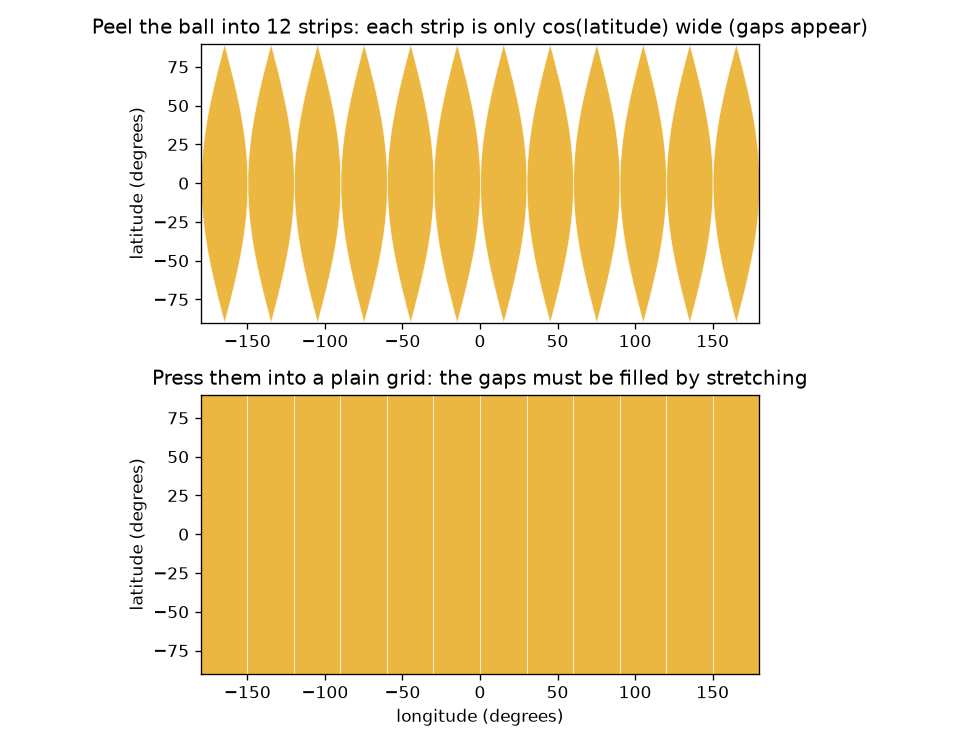
\includegraphics[width=0.85\linewidth]{figures/s01_orange_peel.png}\\\small The peeled ball: strips narrow with latitude, so the plain grid has to stretch them.\end{center}

\subsection*{E. Worked example}
How long is the circle of latitude at 60 degrees north on a ball of radius 6371 km, how long does the flat grid map draw it, and what is the stretch?
\begin{enumerate}[nosep]
\item Equator: 2 pi R = 2 x 3.14159 x 6371 = 40030.2 km. The map draws every circle of latitude with this length.
\item True circle at 60 degrees: 2 pi R cos 60 = 40030.2 x 0.5 = 20015.1 km.
\item Stretch = map length / true length = 40030.2 / 20015.1 = 2.000. This is 1 / cos 60 = 1 / 0.5 = 2.
\item One degree of longitude is R x pi/180 = 111.19 km at the equator but only 55.60 km at 60 degrees north; the map draws both as 111.19 km.
\end{enumerate}
\textbf{Answer.} The true circle is 20015.1 km, the map draws 40030.2 km, so east-west lengths and areas are drawn twice too large at 60 degrees north.

\subsection*{F. Questions}
\begin{enumerate}[nosep]
\item \textbf{Conceptual.} Why can the peel of an orange not be pressed flat without tearing or stretching? What does this mean for every flat map of the Earth?
\item \textbf{Numerical.} At 45 degrees north, what is the true length of 10 degrees of longitude, how long does the equirectangular map draw it, and what is the stretch? Use R = 6371 km.
\item \textbf{Graph and simulation interpretation.} In the stretch graph, read the stretch at 60 degrees and at 80 degrees. By how many times does the area of a country of fixed size grow between 60 and 80 degrees on this map?
\item \textbf{Design and optimisation challenge.} A weather office wants a flat grid map of a region in which east-west lengths are never stretched by more than 25 percent. What is the highest latitude the region may reach? What would you do for a region that reaches 70 degrees?
\end{enumerate}

\section{Session 2: The Mercator projection and area exaggeration}

\subsection*{A. Real-world problem}
A sailor wants to steer by a constant compass bearing and draw the course as one straight line on the chart. In 1569 Mercator made such a map, and navigators adopted it. But on it a box around Greenland looks as big as a box around Africa, although Africa is many times larger. How can a map be so useful and so misleading at once, and up to which latitude is it still honest?

\subsection*{B. Concept and theory}
A point at latitude phi and longitude lambda on a sphere of radius R has the 3D position (R cos phi cos lambda, R cos phi sin lambda, R sin phi). The Mercator map uses x = R lambda and y = R ln tan(pi/4 + phi/2). A small step east and a small step north are both enlarged by the same factor sec(phi) = 1 / cos(phi). Equal enlargement in all directions means small shapes and all angles are kept (the map is conformal) and this is why a constant compass bearing is a straight line. But area is enlarged by sec\textasciicircum{}2(phi). A lat/lon box has the true area R\textasciicircum{}2 (lambda2 - lambda1)(sin phi2 - sin phi1), and on the Mercator map the same box is a rectangle of area R\textasciicircum{}2 (lambda2 - lambda1)(psi2 - psi1) with psi = ln tan(pi/4 + phi/2). Compare these two numbers to see the exaggeration. Which projection to use depends on the job: keep angles (navigation, aviation charts), keep areas (population density maps), or keep distances from one centre (polar maps).

\begin{itemize}[nosep]
\item phi, lambda: latitude and longitude (radians)
\item R: radius of the Earth, 6371 km (km)
\item x, y: Mercator position (km)
\item sec(phi): local length scale of Mercator, 1 / cos(phi) (no unit)
\item k: area exaggeration (map area / true area) (no unit)
\item psi: Mercator height, ln tan(pi/4 + phi/2) (no unit)
\end{itemize}

\begin{equation*}
X=R\cos\varphi\cos\lambda,\quad Y=R\cos\varphi\sin\lambda,\quad Z=R\sin\varphi
\end{equation*}

\begin{equation*}
x=R\lambda,\qquad y=R\ln\tan\!\left(\frac{\pi}{4}+\frac{\varphi}{2}\right)
\end{equation*}

\begin{equation*}
h=k_{\text{north}}=\sec\varphi,\qquad \text{area scale}=\sec^2\varphi
\end{equation*}

\begin{equation*}
A_{\text{sphere}}=R^2(\lambda_2-\lambda_1)(\sin\varphi_2-\sin\varphi_1),\qquad A_{\text{Mercator}}=R^2(\lambda_2-\lambda_1)(\psi_2-\psi_1)
\end{equation*}

\begin{equation*}
\varphi_{\max}=\arccos\frac{1}{\sqrt{k}}
\end{equation*}

\begin{center}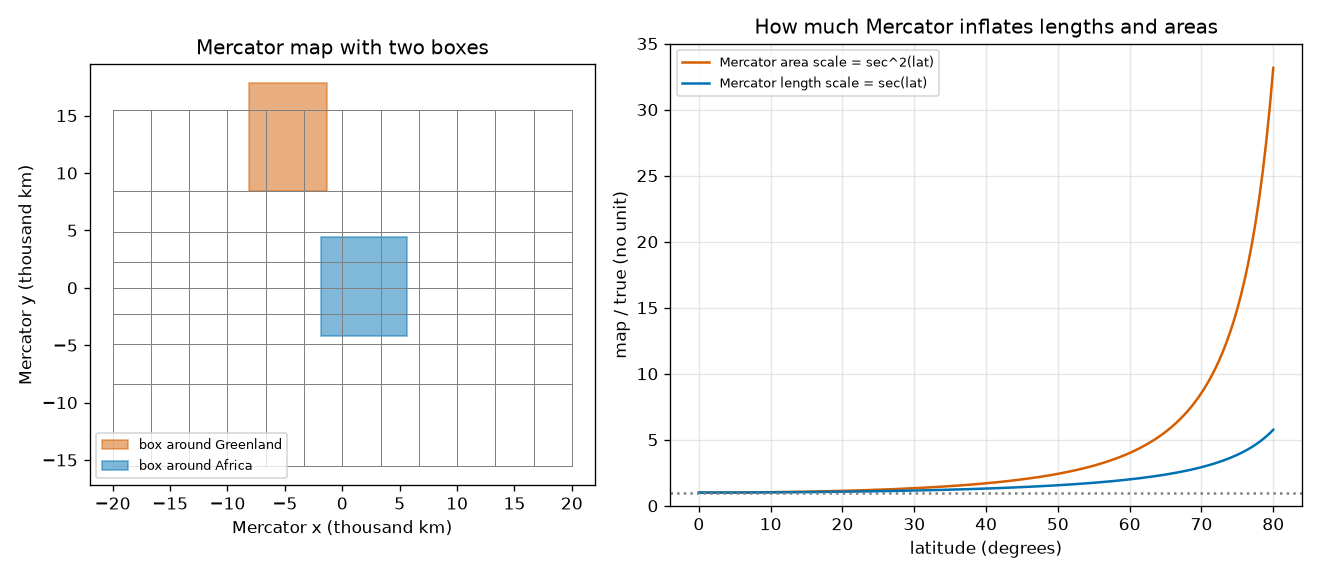
\includegraphics[width=0.85\linewidth]{figures/s02_mercator_exaggeration.png}\\\small Left: a box around Greenland and a box around Africa on a Mercator map. Right: area exaggeration 1 / cos\textasciicircum{}2(latitude) and length scale 1 / cos(latitude).\end{center}

\subsection*{E. Worked example}
Find the Mercator position (x, y) of the point at latitude 60 degrees north and longitude 30 degrees east, its area exaggeration, and the apparent size ratio of the two boxes in Section C.
\begin{enumerate}[nosep]
\item x = R lambda = 6371 x (30 x pi/180) = 6371 x 0.5236 = 3335.8 km.
\item y = R ln tan(45 + 30 degrees) = 6371 x ln tan 75 = 6371 x ln 3.7321 = 6371 x 1.31696 = 8390.3 km.
\item Area exaggeration = 1 / cos\textasciicircum{}2 60 = 1 / 0.25 = 4.0, and the length scale is 2.0.
\item Boxes: true areas are 5.47 million km2 (Greenland box) and 56.62 million km2 (Africa box), a ratio of 10.36. On the Mercator map the box areas are 63.84 and 64.98 million (map) km2, a ratio of only 1.02.
\end{enumerate}
\textbf{Answer.} The point maps to (3335.8, 8390.3) km with area exaggeration 4; the Africa box is truly 10.36 times the Greenland box but the Mercator map shows them almost equal (ratio 1.02).

\subsection*{F. Questions}
\begin{enumerate}[nosep]
\item \textbf{Conceptual.} Why does Mercator keep the shape of small objects but not their area?
\item \textbf{Numerical.} Compute the Mercator coordinates (x, y) in km of the point at latitude 50 degrees north, longitude 10 degrees east, and the area exaggeration there.
\item \textbf{Graph and simulation interpretation.} From the exaggeration curve, at about what latitude does Mercator inflate area by a factor 4, and what is the factor at 80 degrees?
\item \textbf{Design and optimisation challenge.} Design: (1) What latitude limit keeps Mercator's area exaggeration at most 3? (2) Which map property do you need for a world map of population density per square kilometre, for a sea chart, and for a map of the Arctic? Justify each in one line.
\end{enumerate}

\section{Session 3: Measuring distortion with the Jacobian}

\subsection*{A. Real-world problem}
A national mapping agency must choose one projection for its country. Looking at pictures is not enough: it needs numbers for how much each projection stretches lengths, spoils angles and inflates areas at every point. All of this is contained in one small matrix at each point, the Jacobian. Can we compute it for any projection, trust it, and use it to pick the best map for a region and for a purpose?

\subsection*{B. Concept and theory}
A projection sends (latitude phi, longitude lambda) to a map position (x, y). On the unit sphere a small step d(phi) north has length d(phi) and a small step d(lambda) east has length cos(phi) d(lambda). The Jacobian J is the 2 x 2 matrix that turns a tiny ground step (in true length) into a tiny map step: J = [[x\_lambda / cos phi, x\_phi], [y\_lambda / cos phi, y\_phi]]. We estimate each derivative with a central difference f(t + h) - f(t - h) over 2h. A tiny circle on the ground becomes an ellipse (the Tissot indicatrix). Its semi-axes are the singular values s1 \textgreater{}= s2 of J: the largest and the smallest stretch. The area scale is s1 s2 = \textbar{}det J\textbar{}. The angle error is omega = 2 arcsin((s1 - s2)/(s1 + s2)); omega = 0 means the map is conformal and s1 = s2. For the four maps studied here: equirectangular (x = lambda, y = phi) has h = sec phi, k = 1; Mercator has h = k = sec phi; Lambert cylindrical equal-area (x = lambda, y = sin phi) has h = sec phi, k = cos phi, area 1; sinusoidal (x = lambda cos phi, y = phi) has area scale 1. Check: the area of the whole map is the sum of (area scale) x (true cell area cos phi d(phi) d(lambda)); equal-area maps give the area of the sphere, 4 pi R\textasciicircum{}2.

\begin{itemize}[nosep]
\item J: local Jacobian, from true ground length to map length (no unit (R = 1))
\item s1, s2: largest and smallest stretch (singular values of J) (no unit)
\item area scale: s1 x s2 = \textbar{}det J\textbar{}, map area / true area (no unit)
\item omega: largest angle error at the point (degrees)
\item h: finite-difference step (radians (1e-5))
\item R: sphere radius (1 inside the code, 6371 km for the Earth) (km)
\end{itemize}

\begin{equation*}
J=\begin{pmatrix}\dfrac{1}{\cos\varphi}\dfrac{\partial x}{\partial\lambda} & \dfrac{\partial x}{\partial\varphi}\\[2mm] \dfrac{1}{\cos\varphi}\dfrac{\partial y}{\partial\lambda} & \dfrac{\partial y}{\partial\varphi}\end{pmatrix}
\end{equation*}

\begin{equation*}
\frac{\partial f}{\partial t}\approx\frac{f(t+h)-f(t-h)}{2h}
\end{equation*}

\begin{equation*}
s_{1,2}=\text{singular values of }J,\qquad \text{area scale}=s_1s_2=|\det J|
\end{equation*}

\begin{equation*}
\omega=2\arcsin\frac{s_1-s_2}{s_1+s_2}
\end{equation*}

\begin{equation*}
A_{\text{map}}=\iint |\det J|\,\cos\varphi\,d\varphi\,d\lambda\quad(=4\pi R^2\text{ for an equal-area map of the whole sphere})
\end{equation*}

\begin{center}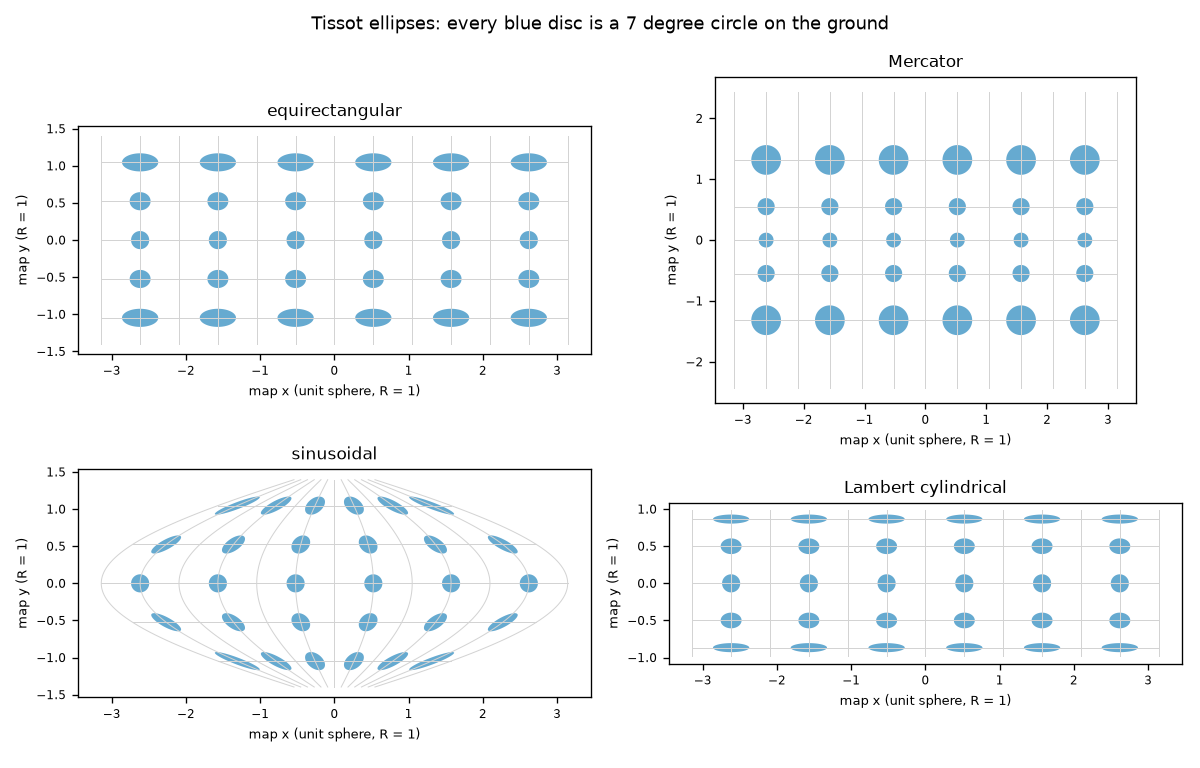
\includegraphics[width=0.85\linewidth]{figures/s03_tissot.png}\\\small Tissot ellipses (7 degree ground circles) for the four projections, drawn from the Jacobian.\end{center}

\subsection*{E. Worked example}
Find the scale factors, area scale and angle error of the Lambert cylindrical equal-area projection at 60 degrees north, by hand and by the finite-difference Jacobian. Then compare the great circle and the Mercator straight line from London (51.5 N, 0.1 W) to New York (40.7 N, 74.0 W).
\begin{enumerate}[nosep]
\item Lambert cylindrical: x = lambda, y = sin phi. So x\_lambda = 1, x\_phi = 0, y\_lambda = 0, y\_phi = cos phi.
\item J = [[1 / cos 60, 0], [0, cos 60]] = [[2, 0], [0, 0.5]]. The singular values are s1 = 2 and s2 = 0.5.
\item Area scale = 2 x 0.5 = 1 (equal-area), and omega = 2 arcsin(1.5 / 2.5) = 2 arcsin(0.6) = 73.74 degrees.
\item The finite-difference Jacobian in Python gives s1 = 2.000, s2 = 0.500, area 1.000, omega 73.74 degrees: the same.
\item Routes (R = 6371 km): great circle 5573 km; the straight line on a Mercator map (constant bearing) is 5797 km, which is 224 km (4.0 percent) longer.
\end{enumerate}
\textbf{Answer.} At 60 N the Lambert cylindrical map has stretches 2 and 0.5, area scale 1 and angle error 73.74 degrees. London to New York is 5573 km by great circle and 5797 km along the Mercator straight line.

\subsection*{F. Questions}
\begin{enumerate}[nosep]
\item \textbf{Conceptual.} A map has an angle error of omega = 0 at every point. What does this say about its Tissot ellipses, and does it say that areas are right?
\item \textbf{Numerical.} For the equirectangular map at 60 degrees north, compute the Jacobian by hand, the area scale and the angle error omega.
\item \textbf{Graph and simulation interpretation.} In the area graph, which projections lie on the line 1 and which do not? What is the reading of the Mercator curve at 80 degrees, and what happens at 90 degrees?
\item \textbf{Design and optimisation challenge.} Design: for a country in lat 8 to 37, lon 68 to 97, you need an equal-area map (area spread at most 1.05). Then, separately, you need a map for navigation (angle error at most 1 degree). Which projection do you choose in each case and what do you give up?
\end{enumerate}

\section{Real-world mini-project}
\textbf{Choose and justify a projection for a country.} Pick a country (or a state, or a sea) and write down its bounding box: a smallest and largest latitude and a smallest and largest longitude, read from any atlas. No data files are needed. Use \texttt{region\_report} from Session 3 to get, for each of the four projections, the worst angle error omega and the area spread (largest area scale divided by smallest). Then decide which property you need (equal areas for a map of population density, kept angles for navigation) and use \texttt{choose\_projection} with a limit that makes sense for your purpose. Example box: lat 8 to 37, lon 68 to 97 (a large Asian country).

\section{The path ahead}
\begin{enumerate}[nosep]
\item \textbf{Session 4: A compromise world map.} A new projection function with a numerical Jacobian, plus a world picture with Tissot ellipses.
\item \textbf{Session 5: A polar map.} An azimuthal map with its own finite-difference distortion table.
\item \textbf{Session 6: A conformal conic map for a country.} A Lambert conformal conic function and a comparison with the four shipped maps.
\item \textbf{Session 7: Routes across the dateline.} A route tool that draws great circles on three projections and reports lengths.
\item \textbf{Session 8: Unroll the globe.} An animation of a globe unrolling into several maps with moving Tissot circles.
\end{enumerate}

\section{Answers and hints}

\subsection*{Session 1}
\begin{enumerate}[nosep]
\item \textbf{Conceptual.} Hint: Compare the length of a circle of latitude on the ball with the width the flat grid gives it. Solution: Near the poles the peel is pinched into narrow strips: a circle of latitude is much shorter than the equator (cos of the latitude times as long). A flat rectangle has the same width at every height, so to fill it the strips must be stretched sideways or you must leave gaps. Any flat map must therefore change some lengths, areas or angles. It cannot be perfect everywhere; you choose which defect to accept.
\item \textbf{Numerical.} Hint: True length = R cos(phi) times the angle in radians; map length = R times the angle in radians. Solution: 10 degrees = 0.17453 radians. True length = 6371 x cos 45 x 0.17453 = 6371 x 0.70711 x 0.17453 = 786.3 km. Map length = 6371 x 0.17453 = 1111.9 km. Stretch = 1111.9 / 786.3 = 1.414 = 1 / cos 45. Sanity check: it lies between 1 (equator) and 2 (60 degrees), as it should.
\item \textbf{Graph and simulation interpretation.} Hint: Area stretch equals east-west stretch on this map. Solution: The curve passes through 2.00 at 60 degrees and 5.76 at 80 degrees. A country of fixed true size therefore looks 5.76 / 2.00 = 2.88 times larger at 80 degrees than at 60 degrees. The curve rises more and more steeply: the map is much worse near the pole than in the middle latitudes.
\item \textbf{Design and optimisation challenge.} Hint: Solve 1 / cos(phi) = 1.25. Solution: cos(phi) = 1 / 1.25 = 0.8, so phi = 36.9 degrees. The region may reach 36.9 degrees north or south. At 70 degrees the stretch is 1 / cos 70 = 2.92, so the plain grid is unsuitable; choose a different projection (Sessions 2 and 3) or a map centred on that latitude. Trade-off: the plain grid is the simplest to compute and plot, but only good near the equator.
\end{enumerate}

\subsection*{Session 2}
\begin{enumerate}[nosep]
\item \textbf{Conceptual.} Hint: Compare the enlargement along the parallel with the enlargement along the meridian, and recall that area is length times width. Solution: At each point Mercator enlarges the east-west and the north-south direction by the same factor sec(phi). Equal enlargement in both directions keeps angles and so the shape of a small object. Area is a product of two lengths, so it is enlarged by sec(phi) times sec(phi) = sec\textasciicircum{}2(phi), which grows quickly toward the poles.
\item \textbf{Numerical.} Hint: x = R lambda; y = R ln tan(pi/4 + phi/2) with phi = 50 degrees, so pi/4 + phi/2 = 70 degrees. Solution: x = 6371 x 0.17453 = 1111.9 km. y = 6371 x ln tan 70 = 6371 x ln 2.7475 = 6371 x 1.0107 = 6439.1 km. Area exaggeration = 1 / cos\textasciicircum{}2 50 = 1 / 0.4132 = 2.42. Sanity check: between 1 (equator) and 4 (60 degrees).
\item \textbf{Graph and simulation interpretation.} Hint: Solve 1 / cos\textasciicircum{}2(phi) = 4 and read the curve at 80. Solution: cos\textasciicircum{}2 phi = 0.25, so cos phi = 0.5 and phi = 60 degrees. At 80 degrees the curve gives 33.2. So a country at 80 degrees looks 33 times too big, compared with 4 times at 60 degrees: the exaggeration explodes toward the poles.
\item \textbf{Design and optimisation challenge.} Hint: Use phi\_max = arccos(1 / sqrt(k)) for part 1. Solution: (1) cos phi = 1 / sqrt(3) = 0.5774, phi = 54.7 degrees. Within 54.7 degrees of the equator the exaggeration is at most 3 (at most 2 within 45 degrees). (2) Population density needs equal areas, because density is people divided by area and the area must be right. A sea chart needs angles kept (conformal) so a compass bearing is a straight line: Mercator. The Arctic is best drawn with a map centred on the pole (azimuthal), because Mercator cannot show the pole at all. This is general guidance; real mapmakers also weigh familiarity and cost.
\end{enumerate}

\subsection*{Session 3}
\begin{enumerate}[nosep]
\item \textbf{Conceptual.} Hint: Look at the two singular values s1 and s2. Solution: omega = 0 means s1 = s2, so every Tissot ellipse is a circle: shapes of small things are kept (conformal). It says nothing about the size: the circles may be bigger or smaller than the ground circle. Mercator is conformal and its circles swell by sec(phi). A map of a sphere cannot be both conformal and equal-area.
\item \textbf{Numerical.} Hint: J = [[sec phi, 0], [0, 1]]; use omega = 2 arcsin((s1 - s2)/(s1 + s2)). Solution: x = lambda, y = phi gives J = [[2, 0], [0, 1]] at 60 degrees, so s1 = 2, s2 = 1. Area scale = 2. omega = 2 arcsin(1/3) = 2 x 19.47 = 38.94 degrees. Sanity check: the area scale 2 equals the Session 1 result sec 60 = 2.
\item \textbf{Graph and simulation interpretation.} Hint: Check the curves of the sinusoidal and Lambert cylindrical maps. Solution: The sinusoidal and Lambert cylindrical maps lie on 1 (equal-area). The equirectangular curve is 1 / cos(phi) (5.76 at 80 degrees) and Mercator is 1 / cos\textasciicircum{}2(phi), which reads 33.2 at 80 degrees. At 90 degrees the Mercator value is infinite: the map cannot show the pole and the Jacobian is undefined there. At 89.9 degrees the value is already 328,285.
\item \textbf{Design and optimisation challenge.} Hint: Use region\_report(8, 37, 68, 97) and choose\_projection. Solution: The report gives (worst omega in degrees, area spread): equirectangular (12.9, 1.24), Mercator (0.0, 1.54), sinusoidal (8.7, 1.00), Lambert cylindrical (25.6, 1.00). Equal-area need: sinusoidal (smaller angle error than Lambert, 8.7 versus 25.6 degrees), giving up some shape accuracy. Navigation need: Mercator, giving up area (the largest area scale is 1.54 times the smallest). Trade-off: no single projection here satisfies both limits, which is why countries often use a different (conic) projection.
\end{enumerate}

\section{How to join}
Read \texttt{CONTRIBUTING.md} in the repository, then pick an issue labelled \texttt{good first issue}. Repository: \url{https://github.com/KrunalPanchal1995/openmapproject}

\end{document}
